\documentclass{article}
\usepackage{arxiv}
\usepackage[utf8]{inputenc} % allow utf-8 input
\usepackage[T1]{fontenc}    % use 8-bit T1 fonts
\usepackage{hyperref}       % hyperlinks
\usepackage{url}            % simple URL typesetting
\usepackage{booktabs}       % professional-quality tables
\usepackage{amsfonts}       % blackboard math symbols
\usepackage{nicefrac}       % compact symbols for 1/2, etc.
\usepackage{microtype}      % microtypography
\usepackage{lipsum}
\usepackage{graphicx}
\usepackage{subcaption}
\usepackage{amsmath}
\usepackage[numbers]{natbib}
\usepackage{float}
\usepackage[nottoc]{tocbibind}

% font size changed from default 10pt to 11pt

\title{A Spatial Analysis of Housing Prices and Supermarket Amenities in London}

\author{
  \large{Kengo Arao}\thanks{With heartfelt thanks to Dr David Candon for dedicated supervision and to Dr Andrei Potlogea for guidance in urban economics}      \thanks{Data and code for this paper are publicly available at \href{https://github.com/KengoA/spatial-analysis-london}{https://github.com/KengoA/spatial-analysis-london}} \\
  Exam Number: B059089 \\
  School of Economics\\
  The University of Edinburgh\\
  \texttt{kengoarao@outlook.com}
}

\begin{document}
\maketitle

\begin{abstract}
Integrating the bid rent theory by Alonso (1964), Muth (1969), and Mills (1972) into the hedonic pricing model by Rosen (1974), I analyse the dynamics of housing prices in Greater London by constructing novel spatial features from Uber Movement and OpenStreetMap. I estimate the commuting cost and find that the average travelling time on the road in the morning has a larger effect on housing prices than geometric distance to the Central Business District, while the latter has a higher explanatory power overall. I then introduce heterogeneity in local amenities and investigate the effects of supermarket amenities, controlling for land use, food and beverage establishments, nature and tourism amenities, and access to education. Through cross-sectional analysis, I find that the presence of high-end supermarkets such as Waitrose and Marks and Spencer is positively associated with higher mean housing prices in a given area, whereas discount stores such as Aldi and Lidl have negative coefficients. Using planning permissions and retail floor spaces as instruments, I provide causal evidence that different classes of supermarkets have opposing effects on housing prices. 

\end{abstract}

% keywords can be removed
% \keywords{First keyword \and Second keyword \and More}
\begin{center}
    \textbf{Word Count}: 10,000
\end{center}

\newpage
\tableofcontents


\newpage
\section{Introduction} \label{section:intro}
In every metropolitan area, housing price has a strong influence over individual consumption choices and hence important implications in social mobility and quality of life. In light of the rapid urbanisation with 68\% of the world population expected to live in urban areas by 2050 (United Nations, 2018), the underlying mechanism of urban housing markets has been under heavy scrutiny in the fields of urban research and economic geography, as well as being a focal point of major media outlets in the United Kingdom (The Guardian, 2019). One particular example of dynamically changing urban landscapes is the penetration of German supermarkets into the British grocery market in recent years (Davey, 2018), with their low-price policies affecting local consumption behaviours. On the other end of the continuum in terms of price levels, several newspaper articles popularised the term "the Waitrose effect" based on a report by Lloyds Bank (2016), which states that proximity to a high-end supermarket such as Waitrose implies a premium on housing prices upwards of 43,000 pound sterling (The Telegraph, 2016; The Independent, 2017). The causal link between the twe and the importance of neighbourhood characteristics on housing prices, nonetheless, remain to be understood with limited literature especially in the United Kingdom. 

The objective of this paper is thus to investigate the effects of such supermarkets and neighbourhood amenities on housing prices at the local level, using empirical models inspired by the bid rent theory by Alonso (1964), Muth (1969) and Mills (1972) for the commuting cost to the Central Business District (CBD) and the hedonic pricing model by Rosen (1974) for product differentiation with objective characteristics. In doing so, I provide novelty in two respects. The first is construction of local amenity variables from OpenStreetMap, an open-sourced collaborative mapping project, which is applicable beyond the scope of the Greater London Area that my empirical analysis is concerned with. The second is the causal analysis of supermarket amenities in the United Kingdom in relation to housing prices with instrumental variables, in which I demonstrate that the presence of high-end supermarkets such as Waitrose and Marks and Spencer cause higher housing prices, controlling for other local amenities and distance to the CBD.

This paper is structured as follows. Section \ref{section:lit} first provides the theoretical foundations of seminal models by Alonso (1964) and Rosen (1974) and discusses the monocentricity assumption in the literature in general and in the context of London, as well as a review of research into local amenities that affect housing prices such as education and consumption accessibility. Section \ref{section:data} briefly describes data sources and their properties, followed by Section \ref{section:variables} where I illustrate data transformation and feature engineering methods. Section \ref{section:model} describes regression models and the results in accordance with the theoretical framework, and provide causal analysis with instrumental variables for high-end and low-end supermarkets. Section \ref{section:discussion} discusses limitations and external validity of this study, and Section \ref{section:conclusion} concludes.


\section{Conceptual Frameworks and Literature Review} \label{section:lit}
This section introduces two theories that are fundamental to the empirical models I develop in Section \ref{section:model}. Each theory is accompanied by a review of empirical research and their implications to this study. [need more words]

\subsection{Bid Rent Theory} \label{subsection:monocentric}
A starting point for understanding urban complexity is a geographic economic theory by Alonso (1964), Muth (1969), and Mills (1972) called bid-rent theory, which refers to the relationship between the distance from the the city centre and real estate price. The basic intuition is that the housing price increases as you move closer towards the CBD, and consumers face a trade-off between housing costs and commuting costs. A simple version of this model described below, the monocentric city model, underpins the empirical specifications throughout this paper and requires the following five assumptions, the first of which will be relaxed in Section \ref{subsection:hedonic}.
\begin{itemize}
\setlength\itemsep{0.1em}
\item Residents are homogeneous and live in a featureless urban area where all the jobs are located in the CBD
\item Each resident is a worker and commutes to a job in the CBD
\item Each worker receives an urban wage $w$ with inelastic labour supply
\item Commuting from distance $d$ entails a linear commuting cost $t(d) = \tau d$
\item Each worker consumes 1 unit of housing which is produced solely  with land
\end{itemize}
Let $p_H (d)$ denote the price of housing located at distance $d$ from the CBD, then a worker's preference can be written as a linear utility function:
\begin{center}
$u = w - p _ { H } ( d ) - t ( d ) = w - p _ { H } ( d ) - \tau d$
\end{center}
With an outside option in the hinterland $\overline{u}$, the spatial equilibrium requires
\begin{center}
$u = w - p _ { H } ( d ) - \tau d = \overline { u }$
\end{center}
Rearranging and partially differentiating $p_H (d)$ with respect to $d$ yields 
\begin{center}
$\frac { \partial p _ { H } ( d ) } { \partial d } = t ^ { \prime } ( d ) = - \tau \quad \forall d \leq \overline { d }$
\end{center}
Let $\overline{d}$ be the upper bound for distance and $\underline{r} > 0$ be the rent for alternative use of land. Then, the equilibrium rent can be written as:

\begin{center}
$p _ { H } ( d ) = \underline { r } + \int _ { d } ^ { \overline { d } } t ^ { \prime } ( \delta ) d \delta = \underline { r } + \tau ( \overline { d } - d )$
\end{center}
Since the alternative land rent $\underline{r}$ is difficult to estimate in practice, I flip the sign of the equation such that 
\begin{center}
$p _ { H } ( d ) = \overline { r } - \int _ { \underline { d } } ^ { d } t ^ { \prime } ( \delta ) d \delta = \overline { r } - \tau ( d - \underline { d } )$
\end{center}
where $\overline{r}$ is the rent in the CBD and $\underline{d}$ is the lower bound for distance, which is 0 at the CBD. This equation hence represents a function of the price of housing which is linearly decreasing in distance from the CBD $d$, which is simply
\begin{center}
$p _ { H } ( d ) = \overline { r } - \tau d$
\end{center}
This will be the basis of the univariate regression models where I estimate the coefficient $\tau$ associated with two measures of distance between the CBD and a given area; orthodromic distance and commuting time cost approximated by Uber Movement Data (Uber Movement, 2019). $\overline{r}$ is the constant term which represents the rent in the CBD at distance $d = 0$.

\subsection{Validity of Monocentricity} \label{subsection:monocentricity}
Bid rent theory remains heavily influential in empirical investigations in urban economics, and location has been a dominant explanatory factor for housing prices and urban structures. However, the assumption of monocentric cities has been actively contested both in theoretical and empirical terms. Fujita and Ogawa (1982) criticise the \textit{a priori} location of the CBD, and provide general equilibrium models where employment centres are endogenously determined by firms and agents.
From an empirical point of view, McMillen (2001) highlights the rise of polycentric city structures in the United States, and identifies employment subcenters in Milwaukee, where employment opportunities are scattered around across the metropolitan area with only 6.7\% of them located in the CBD. A more systematic study is conducted by Arribas-Bel and Sanz-Gracia (2014). They analyse the time trend of high employment density in 359 U.S. metropolitan areas in 1990, 2000, and 2010, and find that employment centres are still largely concentrated centrally, with 57\% of all metropolitan areas exhibiting monocentric structures in 2010. It is noteworthy that there is a large variance in employment share figures in these studies, depending on the definition and scope of the CBD. In general, while there is an increasing number of empirical studies that showcase the polycentric urban structures, the assumption of single-core centres appears to hold across modern metropolitan areas. 

In the context of London, European Commission (1999) describes London as a monocentric city given the strong transport connectivity to the periphery areas and concentration of economic activities in the city. On the other hand, there is limited yet meaningful evidence of the polycentric nature of London. Utilising the large scale data of Oyster card transactions in the London subway, Roth et al. (2011) investigate the individual intraurban flows with the Tube network to identify several basins of attraction in London, the largest of which is West End followed by the City of London area. Importantly, they also demonstrate the significance of the Docklands area where a number of financial firms are located. Similarly, Park (2011) studies commuting flows based on labour market statistics, and identifies a cluster of employment in Westminster, Camden and the City areas. Despite the evidence of heterogeneity especially within the central London, the monocentric structure seems to be present in the scale of Greater London. Hence, this paper follows Park (2011) and impose Alonso's (1964) assumption of monocentricity in examining London's urban structure. Identification of the CBD is further explored in Section \ref{subsection:CBD}.

\subsection{Hedonic Pricing Model and Heterogeneous Amenities} \label{subsection:hedonic} 
In the simple monocentric model, it was assumed that the city is a featureless plane without any urban amenities such as restaurants and cafes. This assumption is now relaxed by introducing heterogeneity in amenities where each subsection of the city has its own characteristics that residents assign specific values to. This is an extension of the hedonic pricing model by Rosen (1974) where a product is valued by its internal characteristics and external factors that are both homogeneous and objective. In Rosen's model, the class of products offers a package of quantifiable characteristics represented by a vector 

\begin{center}
    $z = \left( z _ { 1 } , z _ { 2 } , \dots , z _ { n } \right)$
\end{center}

where $z_i$ is the $i$-th characteristic on a plane of features, which in our case corresponds to the amount of a certain amenity that is present in the neighbourhood. Importantly, market clearing prices $p(z)$ are determined by consumer tastes and production costs, which equalise across buyers and identify the demand structure:

\begin{center}
    $p ( z ) = p \left( z _ { 1 } , z _ { 2 } , \dots , z _ { n } \right)$
\end{center}

The existence of market equilibrium in pure competition and decomposition of products into attributes $z_i$ is the theoretical grounding of the multivariate regressions of this paper, where the first element is the distance from the CBD and $2, 3, ..., n$-th elements are features based on geographical distributions of urban amenities.

While the hedonic pricing model is often applied for a smaller unit of housing such as a house or a flat, Rosen's criterion for objectivity is better suited for neighbourhood characteristics which this paper primarily investigates as some factors in a individual housing unit such as architectural styles and view from the window could entail heterogeneous preferences that are prone to subjectivity.

\subsection{Literature on Housing, Local Amenities, and Supermarkets} \label{subsection:lit:supermarkets}
Hedonic pricing model is heavily utilised in the study of housing markets. Regarding urban amenities, Niu and Liu (2017) provide several proxies to measure accessibility to key economic activities in modelling urban housing price in Beijing. In addition to the employment centre, they investigate the effects of education, consumption and medical accessibility, and calculate the household demand structure for housing prices. They demonstrate that the employment accessibility has by far the highest importance as an economic activity, followed by education, consumption, and medical services. While their results are limited in statistical significance and the scope, their findings motivate the construction of measures of consumption accessibility through the number of supermarkets, and education accessibility in the form of private schools in Section \ref{subsection:school}. In relation to education, Department for Education (2017) finds that home prices in England have a price premium near the schools in the top 10 percent in terms of standardised test performance, where house prices are higher by 8.0\% for primary schools and 6.4\% for secondary schools, holding everything constant.

Another important aspect of daily consumption accessibility that affects individuals universally across socioeconomic strata is supermarkets. Although peer-reviewed research into the effects of supermarket on housing prices is quite limited and virtually nonexistent in the British context, there is a small literature on Walmart openings in the United States. With their low price policy and "big box" establishments, the largest grocery retailer in the U.S. has been attributed to both positive and negative economic effects. 
Basker and Noel (2009) highlight the downward pressure on local inflation as neighbouring businesses and competitors are forced to lower their prices by 1 to 1.2\%, despite the net positive effect on job creation. Dube et al. (2007) find that a new Walmart store reduces local retail revenue levels by 0.5 to 0.9\% at the county level. In regards to housing markets, Pope and Pope (2015) suggest two channels through which a Walmart store affects property values. On one hand, increased accessibility to shopping in general increases housing prices, which is especially the case in more urban environments (Emrath, 2002). In contrast, they hypothesise that a Walmart store potentially decreases housing prices via negative externalities such as higher levels of congestion, pollution and local crime as well as loss of visual aesthetics. Linden and Rockoff (2008), for instance, demonstrates a causal impact of crime risk in the locality on housing prices. To test whether the benefits of accessibility outweigh the costs of negative externalities, they use hedonic pricing models with fixed effects on housing characteristics, and initially find that the Walmart openings are associated with lower housing prices by 2 to 4\% within 2.5 years of opening. Nonetheless, using a difference-in-difference specification, they show that houses around the new Walmart establishment were sold at a 2 to 3\% higher level than the baseline prices, accounting for fixed effects. Similarly, Barrett (2016) demonstrates that the development of a new Walmart store increases the land prices by 39\%, using difference-in-difference estimators. External validity of these results, however, is subject to multiple threats outside of the United States especially due to the spatial constraint in congested urban areas in Europe.

In the United Kingdom, Lloyds Bank's (2016) report on the housing price premium of different supermarket chains in England and Wales was influential in the British media which led to the popularisation of the term "the Waitrose effect" (The Independent, 2017). Supermarkets in general are associated with positive added values in housing prices in varying degrees, with Waitrose and Sainsbury's having a strong premium of £38,666 and £27,939 on average, followed by Marks and Spencer (£27,1812), Tesco (£22,072), Iceland(£20,034), Coop (£17,904), and Morrisons (£10,558). The lower end of distribution includes discount supermarkets such as Asda, Lidl, and Aldi which have marginal levels of premium at £5,026, £3,926 and £1,333, respectively. This translates into a premium of 10\% for Waitrose and Sainsbury's, while those of Asda, Lidl and Aldi are limited to 1-2\%. However, their method to calculate these figures is deeply problematic, in that they compare the average housing prices between a postcode area where a target supermarket is and an area in the same town where it is not. This approach disregards heterogeneity in amenities in different areas and creates a downward bias to areas without any of the these supermarkets, which makes it difficult to isolate the effects of supermarket amenities especially in densely populated areas such as London. Considering the existing research on Walmart, I will investigate the effects of supermarket amenities in a more rigorous manner by controlling for other key measures of accessibility to economic activities within the framework of Alonso (1964) and Rosen (1974). Given the complexity of urban amenities, I compile and synthesise several datasets from different sources for empirical analyses. In doing so, Section \ref{section:data} first describes the data sources and their properties, followed by Section \ref{section:variables} where I carefully construct variables from these datasets.


\section{Data} \label{section:data}
\subsection{Geographic Boundaries}
The geographic unit for this paper's analysis is based on output areas (OAs) which have been the basis for UK Census since 2001, and are designed to be homogeneous in terms of population sizes and household characteristics (Office for National Statistics, 2019). For compatibility with the housing prices data, an aggregate measure of Middle Layer Super Output Areas (MSOA) is obtained from London Datastore (2015) for the empirical analyses throughout the paper with the population ranging from 5000 to 15000 and number of households from 2000 to 6000, where, in the case of Greater London, there are 984 MSOAs and the average population of 8,346 in 2010 (Greater London Authority, 2014).

\subsection{Housing Prices}
Urban rent in each neighbourhood is approximated by property sales registered with Land Registry (2019) which records property sales at the individual dwelling level. This is aggregated for each MSOA at the end of the calendar year for mean and median prices. Table \ref{table:housing} shows descriptive statistics for mean housing prices for each MSOA for the year of 2018, which clearly shows that the prices are not normally distributed with the mean value almost approaching the 75\% percentile, as this is skewed by significantly high housing prices in West London. Figure \ref{fig:price_distribution} maps the geographical distribution of mean housing prices visually both on raw and the log scale.

\begin{table}[H]
\caption{Descriptive Statistics for Mean Housing Prices (GBP)} 
  \label{table:housing} 
\begin{tabular}{lrrrrrrrr}
\toprule
{} &  count &       mean &        std &       min &       25\% &       50\% &       75\% &        max \\
\midrule
Value &  983.0 &  603715.49 &  387541.06 &  226536.0 &  391267.0 &  495010.0 &  673064.5 &  4416659.0 \\
\bottomrule
\end{tabular}
\end{table}

\begin{figure}[H]
  \centering
  \begin{subfigure}{.45\textwidth}
      \centering
      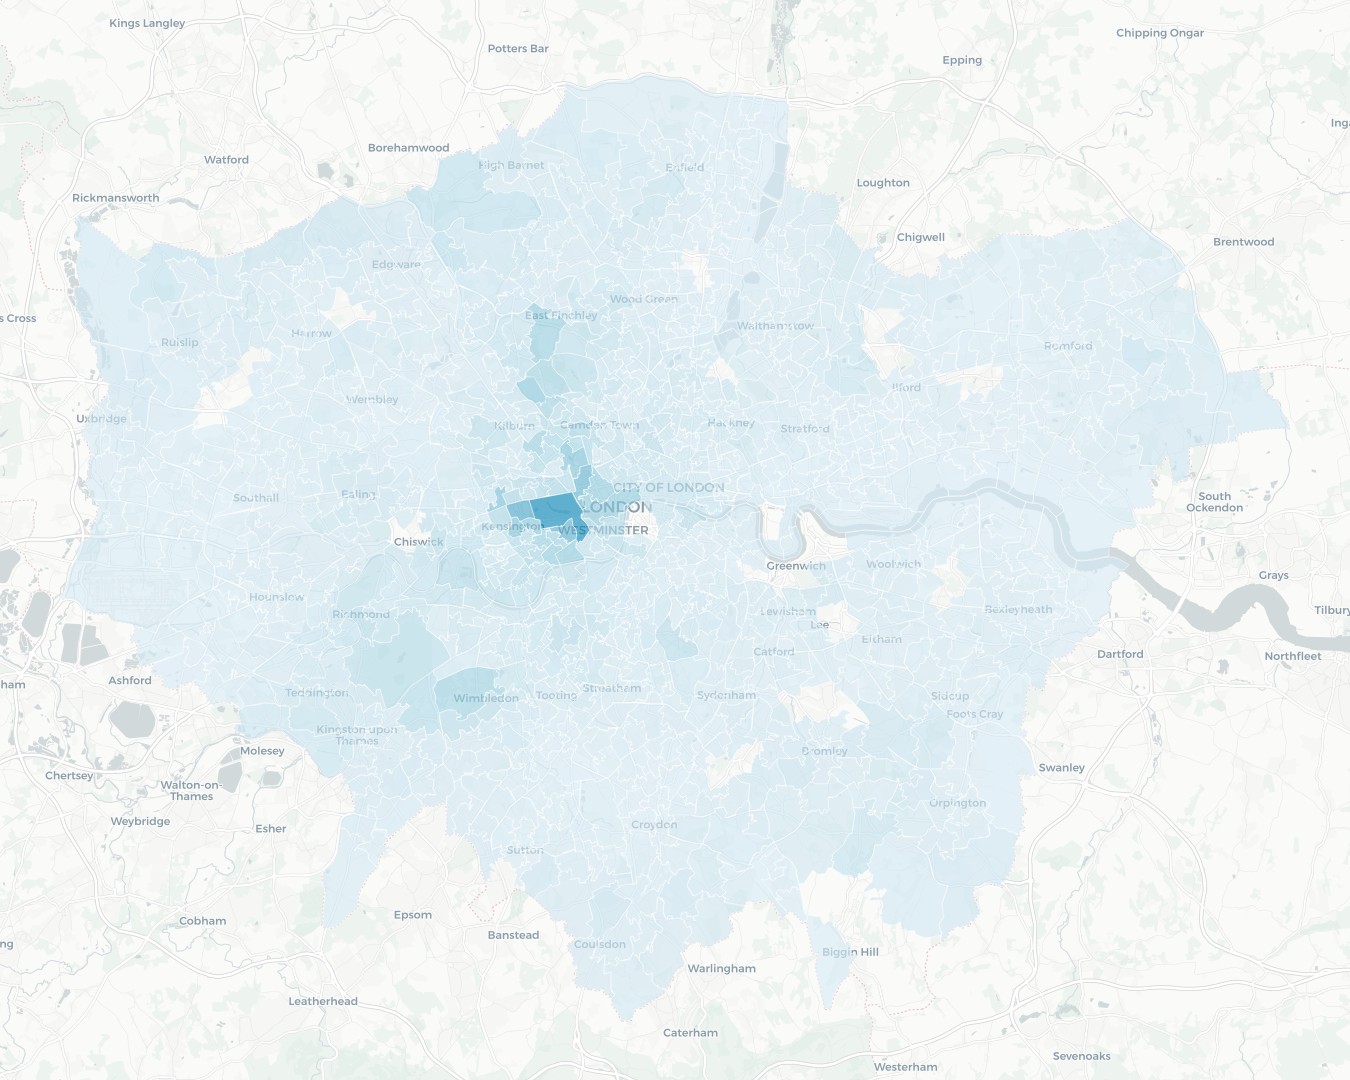
\includegraphics[width=.95\linewidth]{images/housing_raw_mean.png}
      \caption{Mean Housing Price}
      \label{fig:1(a)}
  \end{subfigure}
  \begin{subfigure}{.45\textwidth}
      \centering
      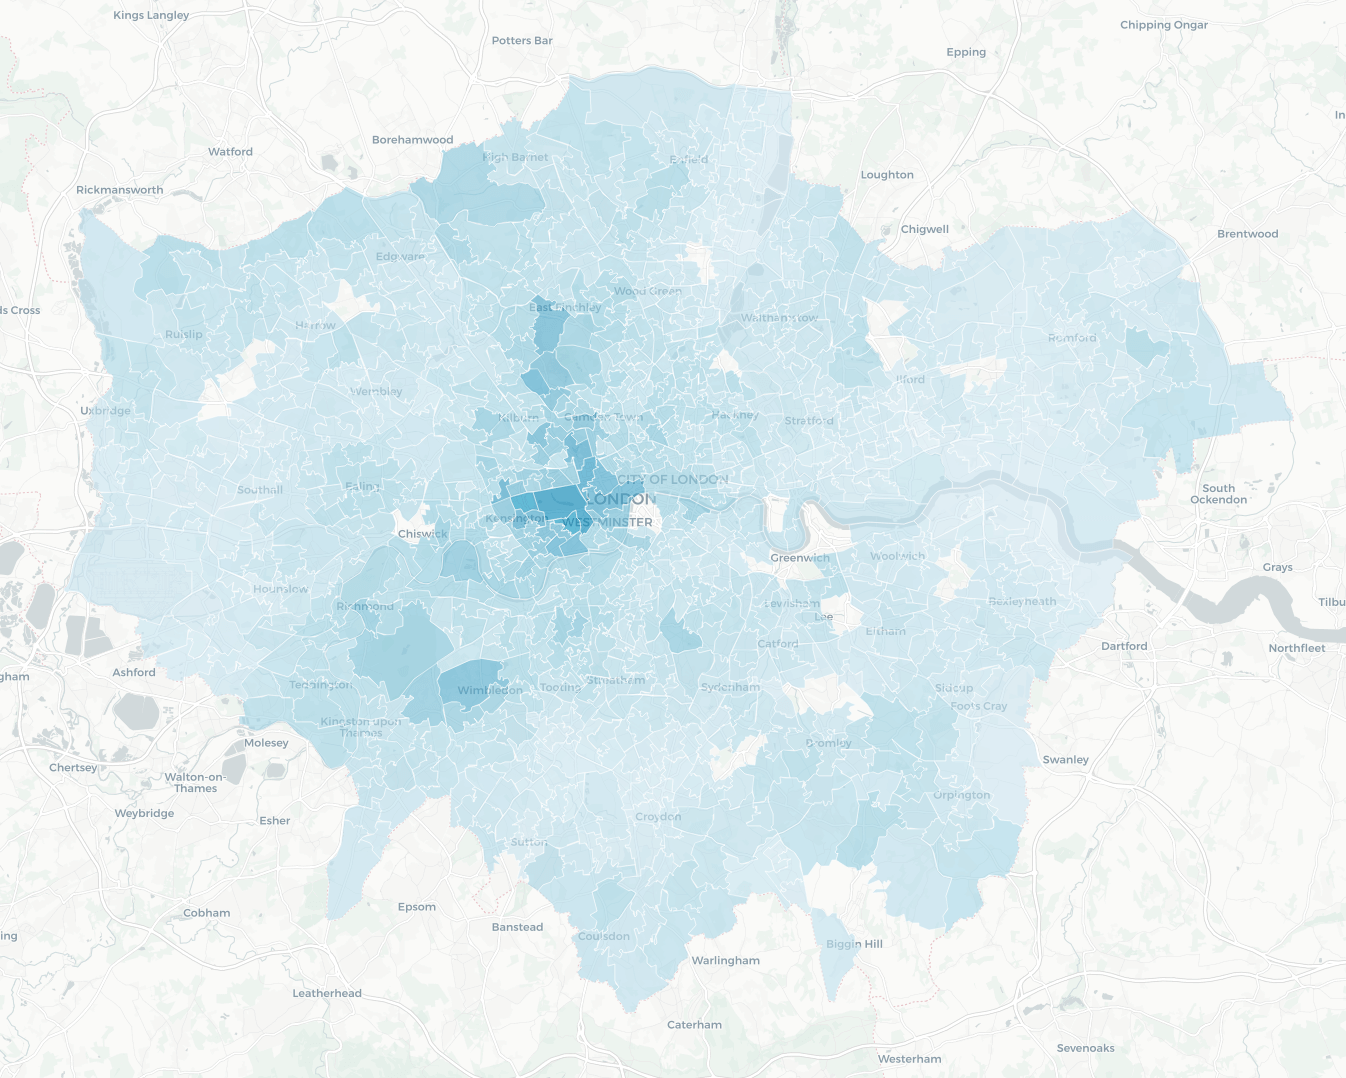
\includegraphics[width=.95\linewidth]{images/housing_log_mean.png}
      \caption{log(Mean Housing Price)}
      \label{fig:1(b)}
  \end{subfigure}
  \caption{Housing Price Distribution Across Greater London}
  \label{fig:price_distribution}
\end{figure}

\subsection{Distance}
Each MSOA is defined as a polygon with edges represented with geographic coordinates of latitudes and longitudes (i.e. Trafalgar Square is at 51.5080 N, 0.1281 W), which will be the basis for the geometric distance measure between each MSOA and the CBD in Section \ref{section:variables}. The second distance measure is morning commuting time on the road, which is approximated from Uber Movement data (2019) that provides anonymised travel data in the form of summary statistics such as mean travel times and standard deviation at a given hour of the day. This data covers major cities in North America, Europe, Australia and India where Uber usage is high, and for Greater London quarterly data is available since 2016.

\subsection{Geographic Information}
The central focus of this paper is the use of geographic features from OpenStreetMap, which is a collaborative mapping scheme launched in 2004. Map data is based on systematic ground surveys by registered contributors.
The crucial feature of this data is the standardised tags that store metadata of the map objects, which come in forms of points, lines, and polygons based on the geographic coordinate system. For instance, an object may consist of key-value pairs of:  \texttt{\{name:'Tesco', building:'supermarket', landuse:'retail'\}} as well as an ordered pair of logtitude and latitude  as coordinates or a vector of coordinates if it is a polygon. Importantly, \texttt{landuse}, \texttt{building} and \texttt{landuse} take standardised values to represent different entities. Other keys that are important are \texttt{type, natural, sport, leisure, historic, tourism, amenity} and \texttt{shop}. I exploit this structure in constructing variables for consumption amenities including supermarkets, in addition to land use and nature controls.

\subsection{Private School Data} \label{subsection:school}
As Niu and Liu (2017) highlighted, accessibility to good schools is an important factor in the household consumption choices of housing. A salient feature of the British educational system is the established presence of private schools that educates 7\% of all children. Ndaji et al. (2016) investigate the difference in educational achievements between independent schools and state schools in the United Kingdom, and demonstrate that students in independent schools had better results by 0.64 GCSE grades, controlling for prior academic ability, socioeconomic disadvantages, and gender differences. This discrepancy is equivalent to additional two years of schooling by the age of 16. Hence, I posit that private school is a desirable education amenity that households with children are especially attracted to. As OpenStreetMap does not provide school type in details, I compile an original dataset for private schools in Greater London in a programmatic manner by scraping a web page by Independent Schools Concil (2019), which provides a comprehensive list of private schools in London providing primary and secondary education. Addresses are then converted into longitudes and latitudes using the \texttt{geocoders.Nominatim} module from \texttt{geopy} library in Python, such that each school falls onto one of the MSOAs.

\section{Variable Construction} \label{section:variables}
Based on the theoretical frameworks and amenities identified in Section \ref{section:lit}, I construct key variables for distance measures and local amenities from data sources introduced in the previous section.
\subsection{Defining the CBD}\label{subsection:CBD}
As Section \ref{subsection:monocentricity} underlined, the exogenous determination of the CBD is a strong assumption in empirical applications of the monocentric city model.  Greater London Authority (2008) qualitatively identifies several sub-centres within inner London (Figure \ref{fig:cbd}). While different CBD functions span horizontally in the north of the River Thames, there appears to be an agglomeration in the West where several industries overlap such as retail, real estate, accounting and consulting, media and creative, and higher education. Park (2011) demonstrates this trend by constructing commuting network into inner London using labour market statistics that records origin-destination trips between local authorities. Figure \ref{fig:park2011} illustrates the commuting patterns in Greater London where the size of each vertex is a linear function of the number of commuting inflows with the direction indicated by an arrow. He identifies a cluster of employment in three boroughs of London as prominent destinations; Camden; Westminster; and the City. Taking these observations into account, this paper assumes  \texttt{Westminster 019}  to be the CBD where London Victoria station is located, that handles a significant amount of traffic inflow as a central London railway terminus with connections to several Tube lines that lead to the city centre. While this does not necessarily reflect the original definition by Alonso (1964) that describes the CBD as an area of workplaces given the small size of the MSOA relative to Greater London, I posit that the commuting inflows and the existence of a transportation hub is a strong indicator of employment accessibility in the modern metropolitan context.


\begin{figure}[H]
\begin{subfigure}{.5\textwidth}
  \centering
  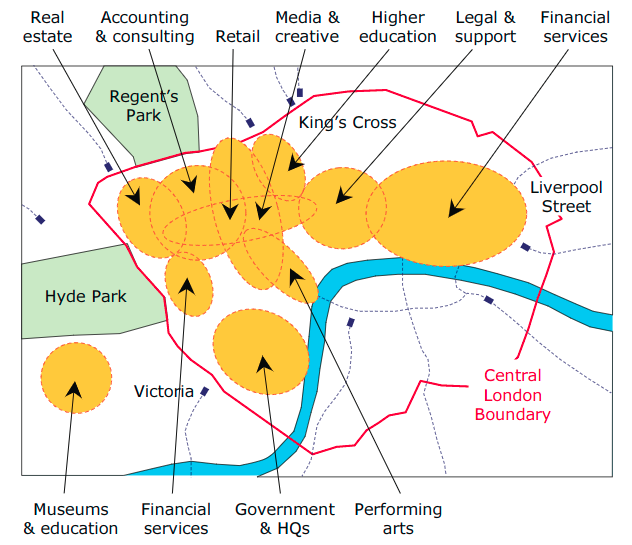
\includegraphics[width=.9\linewidth]{images/cbd.png}
\caption{Distribution of CBD functions (GLA, 2008)}
  \label{fig:cbd}
\end{subfigure}%
\begin{subfigure}{.5\textwidth}
  \centering
  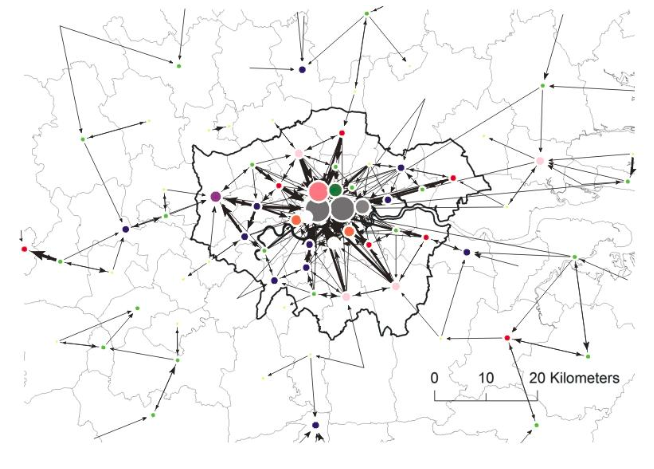
\includegraphics[width=.9\linewidth]{images/park2011.png}
  \caption{Commuting patterns in Greater London (Park, 2011)}
  \label{fig:park2011}
\end{subfigure}
\caption{CBD functions in London}
\label{fig:2}
\end{figure}


\subsection{Distance Measures}
The following illustrates how two measures of distance are constructed. To ensure an approximately normal distribution, both distance measures are log-transformed in the regression models.
\subsubsection{Orthodromic Distance}
The first measure of distance is the distance between two points on a sphere; the centroid of a given area $C_k$ and the centroid of the CBD, $C_0$, which is then converted to miles for ease of interpretation. By construction, each MSOA is represented by a simple polygon where each vertex consists of longitude and latitude in the standard geographic coordinate system (Bolstad, 2016). Let $v_{i,j}$ be a vertex in a N-gon where $v_i$ is a longitude and $v_j$ is a latitude. Then the centroid for a given $k$ is expressed as 

\begin{center}
    $C_k = (C_{ki}, C_{kj})  = (\frac{1}{n} \Sigma_{i=1}^{N} v_i, \frac{1}{n} \Sigma_{j=1}^{N} v_j) $
\end{center}

where $C_{ki}$ and $C_{kj}$ are longitude and latitude for the centroid, respectively. Since the centroids are relatively close to each other with each located in our setting, the Haversine formula (Van Brummelen, 2017) is used for numerical stability to calculate the distance $d$ between two points on a sphere\footnote{The Haversine formula is computationally better conditioned than the arc length formula when two points are close to each other on the sphere due to rounding errors}, $C_0$ and $C_k$, such that

\begin{center}
    $d =2 r \arcsin \left(\sqrt{\sin ^{2}\left(\frac{C_{0i}-C_{ki}}{2}\right)+\cos \left(C_{ki}\right) \cos \left(C_{0i}\right) \sin ^{2}\left(\frac{C_{0j}-C_{kj}}{2}\right)}\right)$
\end{center}
where $r$ is the radius of earth in a desired unit of length, which in this case miles with $r = 3956$. 

\subsubsection{Uber Movement Distance}
To approximate the morning commuting cost, I utilise aggregated Uber Movement data (Uber Movement, 2019) from weekdays in 2017 by calculating the pairwise average time of Uber rides between the CBD and a given MSOA during the AM peak period of 7:00-10:00. It is noteworthy that these two MSOAs do not necessarily have a origin-destination relationship, as Uber's GPS records all subsequent locations from the origin as it traverses through different areas to the final destination (Uber Movement, n.d.). The primary advantage of commuting time measure instead of geometric distance is that it accounts for traffic bottlenecks that stem from terrain structures and road connections. One such instance that demonstrates this advantage with this relatively new dataset is a study by Uber Movement Team (2018) that examines the effect of the closure of the London Tower Bridge. As there is a limited number of bridges across the River Thames, the three-month closure in late 2016 due for structural maintenance led to significantly higher levels of traffic on both sides of the bridge, increasing travel times by up to 65\% for southbound trips and up to 30\% for northbound trips. This variable addresses the problematic assumption of a featureless urban area in the monocentric city model, as it accounts for a nontrivial terrain feature that cuts through the area that is the River Thames in the case of London. 

Figure \ref{fig:price_distribution} demonstrated that the distribution of mean housing prices across MSOAs has a long right tail due to extremely high values around the CBD. Both distance measures constructed in this subsection are also slightly skewed as shown in Table \ref{table:distance} with high values towards the right end of the distribution. The units are miles for \texttt{dist\_miles} and seconds for \texttt{dist\_uber}. Figure \ref{fig:log_log} visualises the log-log linear relationships between these distance measures and mean housing prices. As they allow for interpretation in terms of percentage changes in explanatory and dependent variables, log-scaled values are used for the model specifications in Section \ref{subsection:specifications}.

\begin{table}[H]
\centering
\caption{Descriptive Statistics for Distance Measures} 
  \label{table:distance} 
\begin{tabular}{lrrrrrrrr}
\toprule
{} &  count &     mean &     std &     min &      25\% &      50\% &      75\% &      max \\
\midrule
dist\_miles     &  714.0 &     6.58 &    3.08 &    0.57 &     4.21 &     6.37 &     8.83 &    16.12 \\
dist\_uber &  714.0 &  2151.82 &  815.78 &  183.22 &  1604.15 &  2165.57 &  2730.87 &  4294.00 \\
\bottomrule
\end{tabular}
\end{table}

\begin{figure}[H]
  \begin{subfigure}{.5\textwidth}
      \centering
      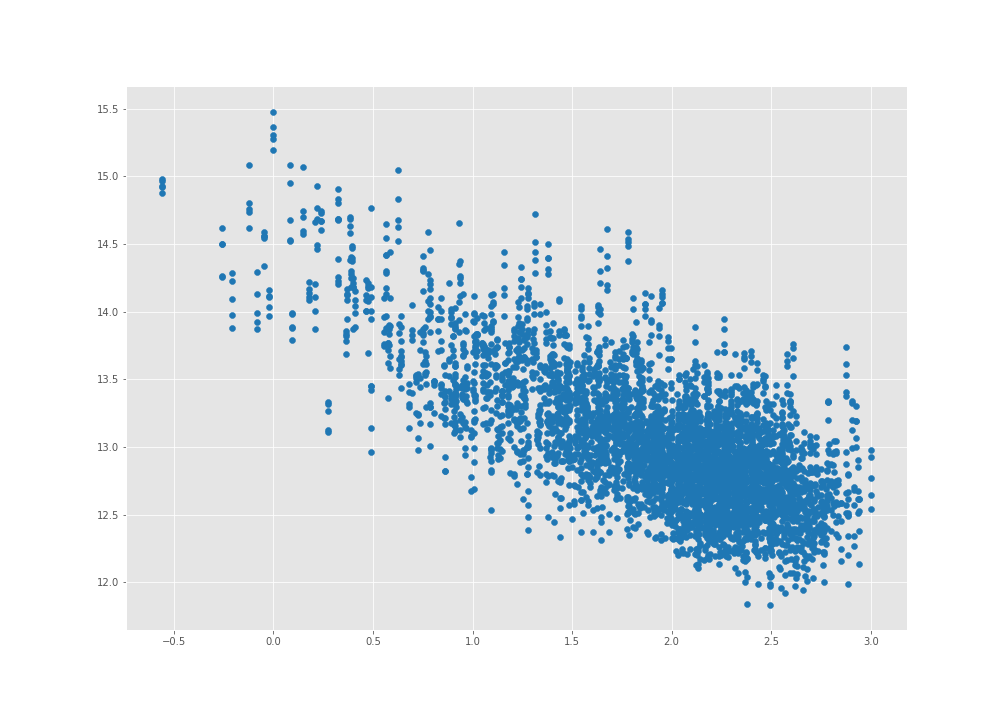
\includegraphics[width=\linewidth]{images/scatter_miles.png}
      \caption{log(Miles distance)}
      \label{fig:3(a)}
  \end{subfigure}
  \begin{subfigure}{.5\textwidth}
      \centering
      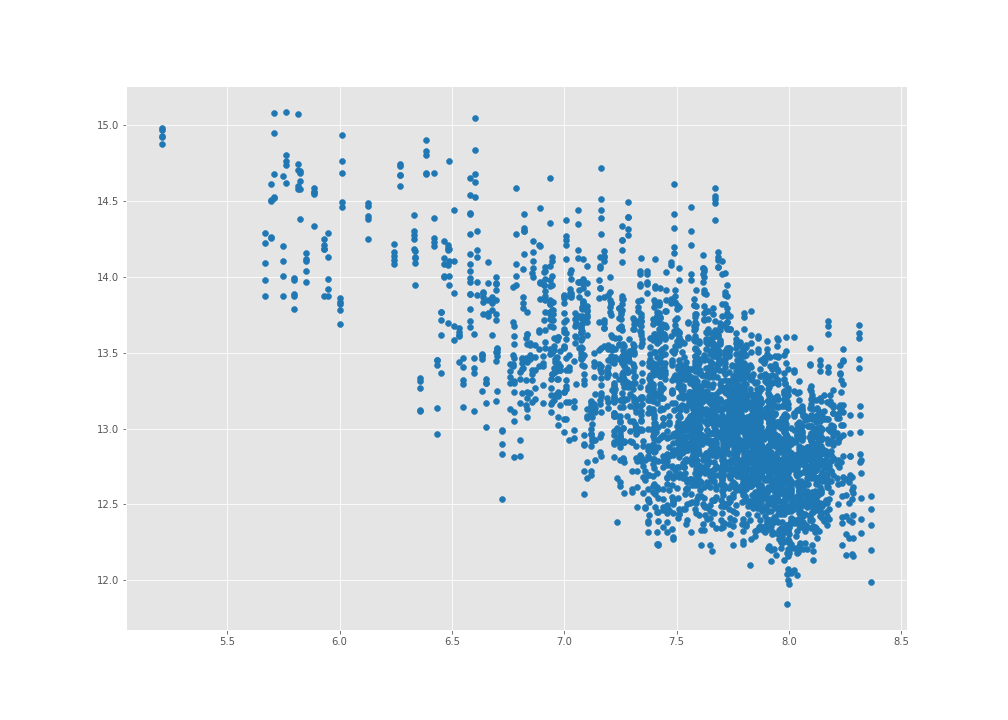
\includegraphics[width=\linewidth]{images/scatter_uber.png}
      \caption{log(Uber Distance in Average Minutes Travelled)}
      \label{fig:3(b)}
  \end{subfigure}
  \caption{Log-log Linearity Between Housing Price and Distance}
  \label{fig:log_log}
\end{figure}

\subsection{Local Amenities from OpenStreetMap}
This section describes the most important novelty of this paper, that is the construction of variables for neighbourhood amenities from OpenStreetMap to characterise modern urban structures. This is followed by introduction of variables used in empirical models in Section \ref{section:model} with reference to existing research on their effects on housing prices. In the hedonic pricing model, local amenities correspond to the vector $z$ that characterises the product, which is the log average housing price of a given MSOA. Among a significant amount of map objects in each area, I utilise \texttt{points} and \texttt{polygons} to construct a variable for each amenity by counting the number of a given entity present in the MSOA. For instance, to construct a variable \texttt{tesco} for a supermarket amenity in the \texttt{City of London 001}, I count the number of occurrences of its standardised name \texttt{Tesco Express, Tesco, Tesco Metro} from each map object within the boundary of \texttt{City of London 001}. To the best of my knowledge, I am the first to utilise these OpenStreetMap objects to represent local amenities as characteristics for housing prices. As I demonstrate in the empirical analysis, they serve as useful approximations for neighbourhood characteristics in terms of land use, nature amenities, and most importantly, consumption amenities that include supermarkets. Nonetheless, this method is not without limitations. First, it implicitly assumes homogeneity within the same class such as \texttt{sainsburys} and \texttt{cafe}, while different establishments might have differing characteristics in reality. Second, there might be a difference between the time an entity, say, a Tesco store, opened and the time it was actually registered as a map object, which is potentially problematic for time series analysis such as difference-in-difference estimators. Potential limitations and their consequences are discussed in detail in Section \ref{subsection:limitations} reflecting on the empirical analysis of the hedonic pricing models. 

As the main interest of this paper, I first construct supermarket amenities. The same supermarket chains are chosen as the report by Lloyds Bank (2016) to investigate their individual effects in Greater London. These are, with variable names in brackets, Waitrose (\texttt{waitrose}), Sainsbury's (\texttt{sainsburys}), Marks and Spencer (\texttt{ms}), Tesco (\texttt{tesco}), Iceland (\texttt{iceland}), Coop (\texttt{coop}), morrisons (\texttt{morrisons}), Asda (\texttt{asda}), Lidl (\texttt{lidl}), and Aldi (\texttt{aldi}). To ensure enough variation and understand a larger trend, this is abstracted to three different categories based on price levels and premium reported in Lloyds (2016), where \texttt{supermarkets\_high} = (\texttt{waitrose, sainsburys, ms}), \texttt{supermarkets\_middle} = (\texttt{tesco, morrisons, coop, iceland}), and \texttt{supermarkets\_low} = (\texttt{asda, lidl, aldi}). Individual effects will also be reported. While OpenStreetMap has a good coverage in terms of the number of establishments for most of these chains, some classes are disproportionately represented such as \texttt{coop} where there are only 13 stores detected across Greater London. Implications of overrepresentation and underrepresentation are discussed in Section \ref{subsubsection:result:hedonic}. These variables alone cannot explain the marginal effects of supermarket amenities as housing price is a function of a number of other characteristics, and empirical models will suffer severely from omitted variable bias. Therefore, the rest of this section outlines key control variables for housing prices that are used in empirical models in Section \ref{section:model}, in addition to the distance measures described above.

To understand the dynamics of housing markets, it is essential to address agent heterogeneity with different preferences for locations. Alonso (1964) argues that offices and commerce are willing to bid the highest rent to secure access to the population in the inner city. On the other hand, manufacturing firms optimise their surplus by choosing to locate in the periphery as they require more land for factories. Figure \ref{fig:landuse} by O'Sullivan (2011) illustrates this trend by considering the interactions between firms and workers. With distance from the CBD on the $x$-axis and urban rent on the $y$-axis, workers follow locations of offices and factories, leading to a second spike in urban rent at a certain distance from the CBD. Since the primary objective of this paper is to understand the implications for household consumption of housing, I consider these variations in firm locations as exogenous and control for the land use effects by introducing \texttt{retail, residential, industrial, construction}, and \texttt{commercial} variables using \texttt{landuse} key from OpenStreetMap.

\begin{figure}[H]
  \centering
  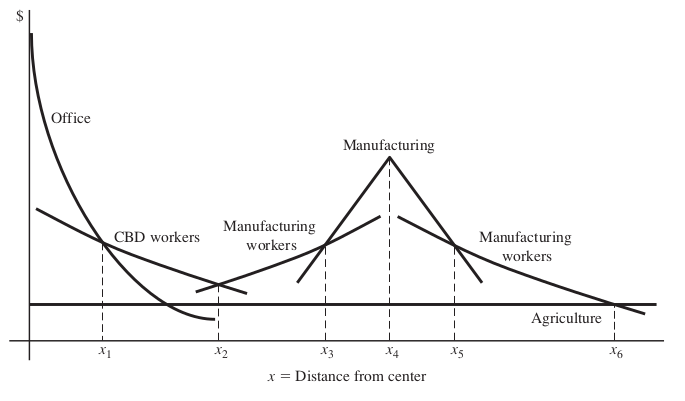
\includegraphics[width=0.8\linewidth]{images/land-use-patterns.png}
  \caption{Land Use Patterns (O'Sullivan, 2011)}
  \label{fig:landuse}
\end{figure}

Another important aspect of London is its popularity among tourists as it attracts by far the largest number of overseas tourists in the United Kingdom (Office for National Statistics, 2019). Studying 103 urban areas in Italy over the 1996-2007 period, Biagi et al. (2015) quantify the influence of tourism-related activities on local housing markets and construct a tourism index that accounts for several amenities such as accommodation and museums, and find that a 1\% increase in tourism index is associated with a 0.2\% increase in housing prices on average as they raise the housing demand, controlling for other population and socioeconomic characteristics in the neighbourhood. While the magnitude of this coefficient appears rather large, it is sensible considering that it is an aggregate index that captures several economic activities in areas where tourism is of particular importance. Office for National Statistics (2013) outlines tourism amenities in the United Kingdom and show that food and beverage serving services has the highest consumption amount in terms of pounds, followed by air passenger transport services, accommodation services, and cultural activities. Reflecting on this, I include tourism control variables under the standardised key \texttt{tourism} from OpenStreetMap that include \texttt{hotel, museum, artwork}, and \texttt{gallery}. Note that food and drink establishments are treated separately from tourism amenities as they also serve the local population, where pubs and restaurants are aggregated as \texttt{pub\_restaurant} due to their high correlation, with other outlets added as \texttt{cafe} and \texttt{fast\_food} based on the \texttt{amenity} key.

In addition, control variables for nature amenities are also considered in terms of green spaces. Gibbons et al. (2014) examine the value of proximity to environmental amenities on property prices in England under a similar hedonic pricing framework at the post code level, while controlling for employment accessibility and labour market characteristics. They find that natural amenities command a premium in housing prices, where gardens, green space such as parks and playgrounds, and areas of water are each associated with a 1\% increase in housing prices for a 1\% increase in terms of land cover share in a given ward.
These effects are partially controlled for by introducing \texttt{garden, pitch, park} and \texttt{playground} from \texttt{leisure} key. However, constructing a variable by counting polygons is not the most suitable measure for nature amenities, given that the variance within each class is likely to be quite large. For instance, Hyde Park should be differentiated from St. James Park due to their size while they might be categorised equally as \texttt{park}. Furthermore, fresh water amenities such as rivers would not be properly represented as they will be a \texttt{line} or a \texttt{multiline} with a vector of coordinates that spans across different areas. For these amenities, land cover shares or proximity to residential areas seem to be a superior method to consider their relationship with housing prices. Nonetheless, for simplicity and consistency, nature controls are added in the same fashion as other variables. Similarly, \texttt{nature\_reserve} and \texttt{golf\_course} are also added under this category as they pertain to the characteristic of large green spaces.

Finally, as studies by Niu and Liu (2017) and Department for Education (2017) showed in Section \ref{subsection:lit:supermarkets}, accessibility to education is crucial for households with children in primary and secondary education. The same variable construction policy is applied to the \texttt{private\_school} data compiled in Section \ref{subsection:school}. While this dataset does not contain the date of establishment, I consider the locations of these schools to be fixed across years given the low frequecny of school relocations and openings, unlike retail stores. I also construct \texttt{school} variable from OpenStreetMap that includes all types of schools as its type is rarely specified in the \texttt{type} key, and test the hypothesis that \texttt{private\_school} is a better proxy for education accessibility that differentiates the quality of education. Higher education is also accounted for with \texttt{university} variable, although this is unlikely to affect housing prices given the lack of generality in location choices of universities.


\section{Empirical Analysis} \label{section:model}
Given the two theoretical frameworks presented in Section \ref{section:lit} and variables constructed in Section \ref{section:variables}, this section first describes empirical strategies using cross-sectional analysis and present the preliminary results. The causal effects of supermarket amenities are then investigated more thoroughly using instrumental variables and first difference estimator, followed by comparisons to existing studies and qualitative analysis.

\subsection{Model Specifications} \label{subsection:specifications}
First of all, the simplest case of the monocentric city model is tested using two distance measures separately. In Section \ref{subsection:monocentric}, I formulated that housing price is a linear function of distance to the CBD, that is, $P_H(d) = \hat{r} - \tau d$, where $\hat{r}$ denotes the rent in the CBD. Considering the log-log linear relationship between distance and housing prices, I run the two following OLS regressions using data from 2018, and estimate two different coefficients for the magnitude of commuting cost $\tau > 0$ for each distance; $\tau_1$ for geometric distance converted to miles and $\tau_2$ for Uber distance approximated by average morning commuting time, such that

\begin{gather*}
ln(P_i) = \hat{r} - \tau_1 ln(dist\_miles_i) + \epsilon_i \\
ln(P_i) = \hat{r} - \tau_2 ln(dist\_uber_i) + \epsilon_i
\end{gather*}
\\
where $P_i$ is the mean housing price for a given MSOA $i$, and $\hat{r}$ corresponds to to the coefficient for the constant term in univariate regressions. Following the analysis on these two specifications, I proceed by adopting one distance measure and setting up a hedonic pricing model to investigate the effects of local amenities introduced in Section \ref{section:variables}. The key explanatory variables here are a vector of supermarkets $\boldsymbol{x}$, which contains three variables aggregated by price levels. Individual effects are also reported by supermarket chains. Adding the local amenities data extracted from 2018 OpenStreetMap data and private school data, the hedonic pricing model is specified as:

\begin{gather*}
ln(P_i) = \hat{r} - \tau ln(dist_i) + \boldsymbol{x_i^{T}} \beta + \boldsymbol{land_i^{T}}\lambda + \boldsymbol{nature_i^{T}} \gamma + \boldsymbol{tourism_i^{T}} \theta + \boldsymbol{food_i^{T}} \phi + \boldsymbol{edu_i^{T}} \mu + \epsilon_i \\
\end{gather*}
such that
\begin{gather*}
\boldsymbol{x} = (supermarkets\_high, supermarkets\_middle, supermarkets\_low) \\
\boldsymbol{land} = (residential, retail, industrial, construction, commercial) \\
\boldsymbol{nature} = (garden, pitch, park, playground, nature\_reserve, golf\_course) \\
\boldsymbol{tourism} = (hotel, atraction, museum, art) \\
\boldsymbol{food} = (pub\_restaurant, cafe, fast\_food) \\ 
\boldsymbol{edu} = (school, private\_school, university) \\ 
\end{gather*}
with each of ($\beta, \lambda, \gamma, \theta, \phi, \mu)$ representing a vector of associated coefficients for amenities within the category.  


\subsection{Results}
\subsubsection{Monocentric City Model}

% Table created by stargazer v.5.2.2 by Marek Hlavac, Harvard University. E-mail: hlavac at fas.harvard.edu
% Date and time: Wed, Mar 27, 2019 - 03:21:58
\begin{table}[H] \centering 
  \caption{Commuting cost comparison} 
  \label{} 
\small 
\begin{tabular}{@{\extracolsep{-10pt}}lcc} 
\\[-1.8ex]\hline 
\hline \\[-1.8ex] 
 & \multicolumn{2}{c}{\textit{Dependent variable:}} \\ 
\cline{2-3} 
\\[-1.8ex] & \multicolumn{2}{c}{log\_price} \\ 
\\[-1.8ex] & (1) & (2)\\ 
\hline \\[-1.8ex] 
 dist\_miles\_log & $-$0.583$^{***}$ &  \\ 
  & (0.021) &  \\ 
  & & \\ 
 dist\_uber\_log &  & $-$0.649$^{***}$ \\ 
  &  & (0.025) \\ 
  & & \\ 
 Constant & 14.299$^{***}$ & 18.197$^{***}$ \\ 
  & (0.038) & (0.193) \\ 
  & & \\ 
\hline \\[-1.8ex] 
Observations & 714 & 714 \\ 
R$^{2}$ & 0.526 & 0.478 \\ 
Adjusted R$^{2}$ & 0.525 & 0.477 \\ 
\hline 
\hline \\[-1.8ex] 
\textit{Note:}  & \multicolumn{2}{r}{$^{*}$p$<$0.1; $^{**}$p$<$0.05; $^{***}$p$<$0.01} \\ 
\end{tabular} 
\end{table} 

I follow Clogg et al. (1995) to examine the difference between the two coefficients $\tau_1$ and $\tau_2$ in two different models, and calculate that $Z = \frac{\tau_1 - \tau_2}{\sqrt{(SE\tau_1)^2 + (SE\tau_2)^2}}  = \frac{-0.583 - (-0.649)}{\sqrt{0.021)^2 + (0.025)^2}} = 2.021$, with $P(Z > 2.021) = 0.022$  which is statistically significant at the 5\% level. 



\subsubsection{Hedonic Pricing Model} \label{subsubsection:result:hedonic}

% Table created by stargazer v.5.2.2 by Marek Hlavac, Harvard University. E-mail: hlavac at fas.harvard.edu
% Date and time: Wed, Mar 27, 2019 - 03:45:07
\begin{table}[H] \centering 
  \caption{Cross-sectional OLS} 
  \label{} 
\small 
\begin{tabular}{@{\extracolsep{-10pt}}lccccccc} 
\\[-1.8ex]\hline 
\hline \\[-1.8ex] 
 & \multicolumn{7}{c}{\textit{Dependent variable:}} \\ 
\cline{2-8} 
\\[-1.8ex] & \multicolumn{7}{c}{log\_price} \\ 
\\[-1.8ex] & (1) & (2) & (3) & (4) & (5) & (6) & (7)\\ 
\hline \\[-1.8ex] 
 dist\_miles\_log & $-$0.513$^{***}$ & $-$0.494$^{***}$ & $-$0.469$^{***}$ & $-$0.486$^{***}$ & $-$0.470$^{***}$ & $-$0.469$^{***}$ & $-$0.440$^{***}$ \\ 
  & (0.015) & (0.015) & (0.015) & (0.015) & (0.015) & (0.015) & (0.015) \\ 
  & & & & & & & \\ 
 supermarkets\_high &  & 0.099$^{***}$ & 0.090$^{***}$ & 0.084$^{***}$ & 0.067$^{***}$ & 0.066$^{***}$ & 0.050$^{***}$ \\ 
  &  & (0.020) & (0.020) & (0.019) & (0.019) & (0.019) & (0.018) \\ 
  & & & & & & & \\ 
 supermarkets\_middle &  & $-$0.024$^{*}$ & $-$0.027$^{**}$ & $-$0.018 & $-$0.019 & $-$0.022$^{*}$ & $-$0.023$^{*}$ \\ 
  &  & (0.012) & (0.013) & (0.012) & (0.013) & (0.013) & (0.012) \\ 
  & & & & & & & \\ 
 supermarkets\_low &  & $-$0.143$^{***}$ & $-$0.116$^{***}$ & $-$0.112$^{***}$ & $-$0.095$^{***}$ & $-$0.093$^{***}$ & $-$0.088$^{***}$ \\ 
  &  & (0.024) & (0.024) & (0.023) & (0.022) & (0.022) & (0.022) \\ 
  & & & & & & & \\ 
%  residential &  &  & 0.009$^{***}$ & 0.007$^{***}$ & 0.008$^{***}$ & 0.008$^{***}$ & 0.007$^{***}$ \\ 
%   &  &  & (0.002) & (0.002) & (0.002) & (0.002) & (0.002) \\ 
%   & & & & & & & \\ 
%  retail &  &  & $-$0.001 & $-$0.0001 & 0.001 & 0.001 & 0.001 \\ 
%   &  &  & (0.002) & (0.002) & (0.002) & (0.002) & (0.002) \\ 
%   & & & & & & & \\ 
%  industrial &  &  & $-$0.031$^{***}$ & $-$0.029$^{***}$ & $-$0.024$^{***}$ & $-$0.024$^{***}$ & $-$0.022$^{***}$ \\ 
%   &  &  & (0.005) & (0.005) & (0.005) & (0.005) & (0.005) \\ 
%   & & & & & & & \\ 
%  construction &  &  & 0.010$^{*}$ & 0.011$^{**}$ & 0.009 & 0.008 & 0.008 \\ 
%   &  &  & (0.005) & (0.005) & (0.005) & (0.005) & (0.005) \\ 
%   & & & & & & & \\ 
%  commercial &  &  & 0.003 & 0.004 & $-$0.019$^{***}$ & $-$0.018$^{***}$ & $-$0.018$^{***}$ \\ 
%   &  &  & (0.005) & (0.005) & (0.006) & (0.006) & (0.006) \\ 
%   & & & & & & & \\ 
%  garden &  &  &  & 0.0004 & 0.0001 & 0.0001 & 0.0002 \\ 
%   &  &  &  & (0.001) & (0.001) & (0.001) & (0.001) \\ 
%   & & & & & & & \\ 
%  pitch &  &  &  & 0.006$^{***}$ & 0.005$^{***}$ & 0.005$^{***}$ & 0.003$^{**}$ \\ 
%   &  &  &  & (0.001) & (0.001) & (0.001) & (0.001) \\ 
%   & & & & & & & \\ 
%  park &  &  &  & $-$0.003 & $-$0.004$^{*}$ & $-$0.004$^{*}$ & $-$0.003$^{*}$ \\ 
%   &  &  &  & (0.002) & (0.002) & (0.002) & (0.002) \\ 
%   & & & & & & & \\ 
%  playground &  &  &  & $-$0.029$^{***}$ & $-$0.028$^{***}$ & $-$0.029$^{***}$ & $-$0.022$^{***}$ \\ 
%   &  &  &  & (0.006) & (0.006) & (0.006) & (0.006) \\ 
%   & & & & & & & \\ 
%  nature\_reserve &  &  &  & 0.006 & 0.016 & 0.015 & 0.035 \\ 
%   &  &  &  & (0.028) & (0.027) & (0.027) & (0.026) \\ 
%   & & & & & & & \\ 
%  golf\_course &  &  &  & 0.194$^{***}$ & 0.185$^{***}$ & 0.180$^{***}$ & 0.144$^{***}$ \\ 
%   &  &  &  & (0.035) & (0.035) & (0.035) & (0.033) \\ 
%   & & & & & & & \\ 
%  hotel &  &  &  &  & $-$0.005 & $-$0.004 & $-$0.004 \\ 
%   &  &  &  &  & (0.004) & (0.004) & (0.004) \\ 
%   & & & & & & & \\ 
%  attraction &  &  &  &  & 0.015$^{*}$ & 0.015$^{*}$ & 0.018$^{**}$ \\ 
%   &  &  &  &  & (0.009) & (0.009) & (0.009) \\ 
%   & & & & & & & \\ 
%  museum &  &  &  &  & 0.037 & 0.037 & 0.021 \\ 
%   &  &  &  &  & (0.029) & (0.029) & (0.028) \\ 
%   & & & & & & & \\ 
%  art &  &  &  &  & 0.027 & 0.027 & $-$0.007 \\ 
%   &  &  &  &  & (0.024) & (0.024) & (0.023) \\ 
%   & & & & & & & \\ 
 pub\_restaurant &  &  &  &  & 0.010$^{***}$ & 0.009$^{***}$ & 0.010$^{***}$ \\ 
  &  &  &  &  & (0.003) & (0.003) & (0.003) \\ 
  & & & & & & & \\ 
 cafe &  &  &  &  & 0.005 & 0.005 & 0.003 \\ 
  &  &  &  &  & (0.006) & (0.006) & (0.005) \\ 
  & & & & & & & \\ 
 fast\_food &  &  &  &  & $-$0.026$^{***}$ & $-$0.026$^{***}$ & $-$0.025$^{***}$ \\ 
  &  &  &  &  & (0.005) & (0.005) & (0.005) \\ 
  & & & & & & & \\ 
 school &  &  &  &  &  & 0.010$^{*}$ &  \\ 
  &  &  &  &  &  & (0.005) &  \\ 
  & & & & & & & \\ 
 private\_school &  &  &  &  &  &  & 0.124$^{***}$ \\ 
  &  &  &  &  &  &  & (0.014) \\ 
  & & & & & & & \\ 
 university &  &  &  &  &  & $-$0.0002 & $-$0.002 \\ 
  &  &  &  &  &  & (0.006) & (0.006) \\ 
  & & & & & & & \\ 
 Controls: Land Use &  & YES & YES  & YES  & YES &  YES & YES \\ 
  &  &  &  &  &  &  & \\ 
 Controls: Nature &  &  &  YES & YES  & YES & YES & YES \\ 
  &  &  &  &  &  &  &  \\ 
 Controls: Tourism &  &  &  & YES & YES & YES & YES  \\ 
  &  &  &  &  &  &  & \\ 
 Constant & 14.330$^{***}$ & 14.300$^{***}$ & 14.230$^{***}$ & 14.260$^{***}$ & 14.220$^{***}$ & 14.200$^{***}$ & 14.140$^{***}$ \\ 
  & (0.035) & (0.036) & (0.037) & (0.037) & (0.038) & (0.039) & (0.037) \\ 
  & & & & & & & \\ 
\hline \\[-1.8ex] 
Observations & 951 & 951 & 951 & 951 & 951 & 951 & 951 \\ 
R$^{2}$ & 0.543 & 0.570 & 0.596 & 0.631 & 0.652 & 0.653 & 0.680 \\ 
Adjusted R$^{2}$ & 0.543 & 0.568 & 0.592 & 0.625 & 0.644 & 0.644 & 0.671 \\ 
\hline 
\hline \\[-1.8ex] 
\textit{Note:}  & \multicolumn{7}{r}{$^{*}$p$<$0.1; $^{**}$p$<$0.05; $^{***}$p$<$0.01} \\ 
\end{tabular}
\end{table}

\begin{table}[H] \centering 
  \caption{Individual Supermarket Effects} 
  \label{} 
\small 
\begin{tabular}{@{\extracolsep{5pt}} ccccccccccc} 
\\[-1.8ex]\hline 
\hline \\[-1.8ex] 
 & waitrose & ms & sainsburys & tesco & iceland & morrisons & coop & lidl & asda & aldi \\ 
\hline \\[-1.8ex]
Count & 124 & 76 & 94 & 526 & 115 & 64 & 13 & 103 & 29 & 50 \\ 
Estimate & $0.052$ & $0.060$ & $0.032$ & $-0.011$ & $-0.056$ & $-0.028$ & $-0.116$ & $-0.102$ & $-0.061$ & $-0.085$ \\ 
Std. Error & $0.030$ & $0.043$ & $0.038$ & $0.015$ & $0.031$ & $0.033$ & $0.085$ & $0.031$ & $0.043$ & $0.055$ \\ 
t-value & $1.705$ & $1.408$ & $0.826$ & $-0.741$ & $-1.812$ & $-0.848$ & $-1.368$ & $-3.281$ & $-1.436$ & $-1.536$ \\ 
Pr(\textgreater \textbar t\textbar ) & $0.088$ & $0.159$ & $0.409$ & $0.459$ & $0.070$ & $0.397$ & $0.172$ & $0.001$ & $0.151$ & $0.125$ \\ 
\hline \\[-1.8ex] 
\end{tabular} 
\end{table} 


\subsection{Causal Analysis of Supermarket Amenities}
    
\subsubsection{Instrumental Variable}
% Table created by stargazer v.5.2.2 by Marek Hlavac, Harvard University. E-mail: hlavac at fas.harvard.edu
% Date and time: Wed, Mar 27, 2019 - 04:24:52
\begin{table}[!htbp] \centering 
  \caption{Instrumental Variables} 
  \label{} 
\begin{tabular}{@{\extracolsep{5pt}}lcc} 
\\[-1.8ex]\hline 
\hline \\[-1.8ex] 
 & \multicolumn{2}{c}{\textit{Dependent variable:}} \\ 
\cline{2-3} 
\\[-1.8ex] & \multicolumn{2}{c}{log\_price} \\ 
\\[-1.8ex] & \textit{OLS} & \textit{IV} \\ 
\\[-1.8ex] & (1) & (2)\\ 
\hline \\[-1.8ex] 
 dist\_miles\_log & $-$0.440$^{***}$ & $-$0.354$^{***}$ \\ 
  & (0.015) & (0.048) \\ 
  & & \\ 
 supermarkets\_high & 0.050$^{***}$ & 0.848$^{**}$ \\ 
  (instrument: planning leniency) & (0.018) & (0.375) \\ 
  & & \\ 
 supermarkets\_middle & $-$0.021$^{*}$ & $-$0.041 \\ 
   & (0.012) & (0.033) \\ 
  & & \\ 
 supermarkets\_low & $-$0.089$^{***}$ & $-$0.643$^{**}$ \\ 
  (instrument: retail area size) & (0.022) & (0.323) \\ 
  & & \\ 
 Constant & 14.140$^{***}$ & 13.920$^{***}$ \\ 
  & (0.037) & (0.127) \\ 
  & & \\ 
\hline \\[-1.8ex] 
Weak instruments (supermarkets\_high) &  & 0.0011*** \\ 
Weak instruments (supermarkets\_low) &  & 0.0000*** \\ 
Wu-Hausman &  & 0.0002*** \\ 
Observations & 951 & 951 \\ 
R$^{2}$ & 0.679 & $-$0.135 \\ 
Adjusted R$^{2}$ & 0.671 & $-$0.165 \\ 
Residual Std. Error (df = 926) & 0.258 & 0.486 \\ 
\hline 
\hline \\[-1.8ex] 
\textit{Note: All other controls are included}  & \multicolumn{2}{r}{$^{*}$p$<$0.1; $^{**}$p$<$0.05; $^{***}$p$<$0.01} \\ 
\end{tabular} 
\end{table} 

\subsubsection{First Difference Estimator}
% Table created by stargazer v.5.2.2 by Marek Hlavac, Harvard University. E-mail: hlavac at fas.harvard.edu
% Date and time: Wed, Mar 27, 2019 - 06:27:15
\begin{table}[H] \centering 
  \caption{First Difference Estimator} 
  \label{} 
\small 
\begin{tabular}{@{\extracolsep{-10pt}}lc} 
\\[-1.8ex]\hline 
\hline \\[-1.8ex] 
 & \multicolumn{1}{c}{\textit{Dependent variable:}} \\ 
\cline{2-2} 
\\[-1.8ex] & lp\_d \\ 
\hline \\[-1.8ex] 
 sh\_d & $-$0.022$^{*}$ \\ 
  & (0.013) \\ 
  & \\ 
 sm\_d & $-$0.016$^{*}$ \\ 
  & (0.009) \\ 
  & \\ 
 sl\_d & 0.004 \\ 
  & (0.014) \\ 
  & \\ 
 Constant & 0.381$^{***}$ \\ 
  & (0.005) \\ 
  & \\ 
\hline \\[-1.8ex] 
Observations & 951 \\ 
R$^{2}$ & 0.007 \\ 
Adjusted R$^{2}$ & 0.004 \\ 
\hline 
\hline \\[-1.8ex] 
\textit{Note:}  & \multicolumn{1}{r}{$^{*}$p$<$0.1; $^{**}$p$<$0.05; $^{***}$p$<$0.01} \\ 
\end{tabular} 
\end{table} 

% Table created by stargazer v.5.2.2 by Marek Hlavac, Harvard University. E-mail: hlavac at fas.harvard.edu
% Date and time: Wed, Mar 27, 2019 - 06:27:46
\begin{table}[H] \centering 
  \caption{Individual FD Effects} 
  \label{} 
\small 
\begin{tabular}{@{\extracolsep{-10pt}} ccccccccccc} 
\\[-1.8ex]\hline 
\hline \\[-1.8ex] 
 & waitrose\_d & ms\_d & sainsburys\_d & tesco\_d & iceland\_d & morrisons\_d & coop\_d & lidl\_d & asda\_d & aldi\_d \\ 
\hline \\[-1.8ex] 
Count (nonzero) & 29 & 25 & 36 & 122 & 39 & 23 & 5 & 32 & 18 & 14 \\ 
Estimate & $-0.095$ & $-0.019$ & $0.032$ & $-0.021$ & $0.022$ & $-0.038$ & $0.015$ & $-0.022$ & $0.028$ & $0.005$ \\ 
Std. Error & $0.022$ & $0.026$ & $0.023$ & $0.011$ & $0.020$ & $0.026$ & $0.060$ & $0.021$ & $0.028$ & $0.033$ \\ 
t-value & $-4.292$ & $-0.718$ & $1.419$ & $-1.883$ & $1.066$ & $-1.424$ & $0.243$ & $-1.023$ & $1.004$ & $0.158$ \\ 
Pr(\textgreater \textbar t\textbar ) & $0.00002$ & $0.473$ & $0.156$ & $0.060$ & $0.287$ & $0.155$ & $0.808$ & $0.306$ & $0.315$ & $0.875$ \\ 
\hline \\[-1.8ex] 
\end{tabular} 
\end{table}


low coefficient sensible

no rigorous DID such as Pope and Pope (2015) and Barrett (2016)

lack of data for opening, announcement and closing date
measurement errors from openstreetmap data

higher land prices during development period if its on a new soil
 prices already priced in

converted stores?



    
\section{Discussion} \label{section:discussion}

\subsection{External Validity}
\subsection{Limitations and Future Work} \label{subsection:limitations}

\section{Conclusion} \label{section:conclusion}


\newpage
\nocite{*}
\renewcommand\harvardyearleft{\unskip, }
\renewcommand\harvardyearright[1]{.}
\let\oldthebibliography\thebibliography
\renewcommand\thebibliography{\let\bf\relax\oldthebibliography}
\renewcommand{\refname}{\textbf{Bibliography}}
\bibliographystyle{agsm}  
\bibliography{bibliography.bib}

\end{document}